% Lecture Template for ME3023 -  Measurements in Mechanical Systems - Tennessee Technological University
% Spring 2020 - Summer 2020 - Fall 2020 - Spring 2021 - Summer 2021
% Tristan Hill, May 07, 2020 - June 12, 2020 - July 08, 2020 - Novemeber 02, 2020 - March 28, 2021 - May 25, 2021 - August 21, 2022

% Fall 2023 - condensing and streamlining lectures by combining topics into a single PDF under the module name
%			  this will simplify file and link management as well as make lectures easier to use in class
%			- added image/ to clean directory and reduce redundancy, specific to module for now  

% Module Name: Dimensional Instruments
% Topic 1 - Using Calipers
% Topic 2 - Using Micrometers 

\documentclass[fleqn]{beamer} % for presentation (has nav buttons at bottom)


%\usepackage{/mnt/c/Users/thill/Documents/courses/measurements/lectures/measurements_lectures}

\usepackage{/home/tntech.edu/thill/courses/measurements/lectures/measurements_lectures}


\author{ME3023 - Measurements in Mechanical Systems} % original formatting from Mike Renfro, September 21, 2004

\newcommand{\MNUM}{2\hspace{2mm}} % module number 
\newcommand{\moduletitle}{Dimensional Instruments}
%\newcommand{\topictitle}{General Measurement System} 

\newcommand{\sectionItitle}{Using Calipers}
\newcommand{\sectionIItitle}{Using Micrometers}

\newcommand{\sectionIsubsectionItitle}{Overview}
\newcommand{\sectionIsubsectionIItitle}{Components}
\newcommand{\sectionIsubsectionIIItitle}{Vernier Calipers}
\newcommand{\sectionIsubsectionIVtitle}{Digital Calipers}
\newcommand{\sectionIsubsectionVtitle}{Group Activity}

\newcommand{\sectionIIsubsectionItitle}{Overview}
\newcommand{\sectionIIsubsectionIItitle}{Components}
\newcommand{\sectionIIsubsectionIIItitle}{Vernier Micrometer}
\newcommand{\sectionIIsubsectionIVtitle}{Digital Micrometer}

% custom box
\newsavebox{\mybox}

\title{Lecture Module - \moduletitle}

\date{Mechanical Engineering\vspc Tennessee Technological University}

\begin{document}

	\lstset{language=MATLAB,basicstyle=\ttfamily\small,showstringspaces=false}

	\frame{\titlepage \center\begin{framed}\Large \textbf{Module \MNUM - \moduletitle}\end{framed} \vspace{5mm}}

	% Module Outline
	\begin{frame} 
		\large \textbf{Module \MNUM - \moduletitle} \vspace{3mm}\\

		\begin{itemize}
			\item Topic 1 - \hyperlink{sectionI}{\sectionItitle} \vspc % section I
			\item Topic 2 - \hyperlink{sectionII}{\sectionIItitle} \vspc % section II
			%\item Topic 3 - \hyperlink{sectionIII}{\sectionIIItitle} \vspc % section III
			%\item Topic 4 - \hyperlink{sectionIV}{\sectionIVtitle} \vspc % section IV
		\end{itemize}

	\end{frame}

	% section I
	\section{\sectionItitle}\label{sectionI}

		% section I Outline
		\begin{frame} 
			\large \textbf{Topic 1 - \sectionItitle} \vspace{3mm}\\

			\begin{itemize}
				\item \hyperlink{sectionIsubsectionI}{\sectionIsubsectionItitle} \vspc %  section I subsection I
				\item \hyperlink{sectionIsubsectionII}{\sectionIsubsectionIItitle} \vspc % section I subsection II
				\item \hyperlink{sectionIsubsectionIII}{\sectionIsubsectionIIItitle} \vspc % section I subsection III
				\item \hyperlink{sectionIsubsectionIV}{\sectionIsubsectionIVtitle} \vspc % section I subsection IV
				\item \hyperlink{sectionIsubsectionV}{\sectionIsubsectionVtitle} \vspc % section I subsection V
			\end{itemize}
		\end{frame}
		
		% section I subsection I 
		\subsection{\sectionIsubsectionItitle}\label{sectionIsubsectionI}

			\begin{frame}
				\frametitle{\sectionIsubsectionItitle}
				\begin{itemize}

					\item A caliper ( ... a pair of calipers) is a device used to measure the distance between two opposite sides of an object. {\tiny Text: \href{https://en.wikipedia.org/wiki/Calipers}{Wikipedia}}
					\begin{itemize}

						\item Length, Width, Height
						\item Inside and Outside Diameter
						\item Depth 

					\end{itemize}

					\vspace{5mm}
					\item There is a wide variety of caliper(s). This word means different things in different fields. 
					\begin{itemize}

						\item Engineering and Deisgn
						\item Machining and Construction
						\item Medical Applications and Others

					\end{itemize}

				\end{itemize}

			\end{frame}

		% section I subsection II
		\subsection{\sectionIsubsectionIItitle}\label{sectionIsubsectionII}

			\begin{frame}
				\frametitle{\sectionIsubsectionIItitle}

				{\tiny Text: \href{https://en.wikipedia.org/wiki/Vernier_scale}{Wikipedia}}

				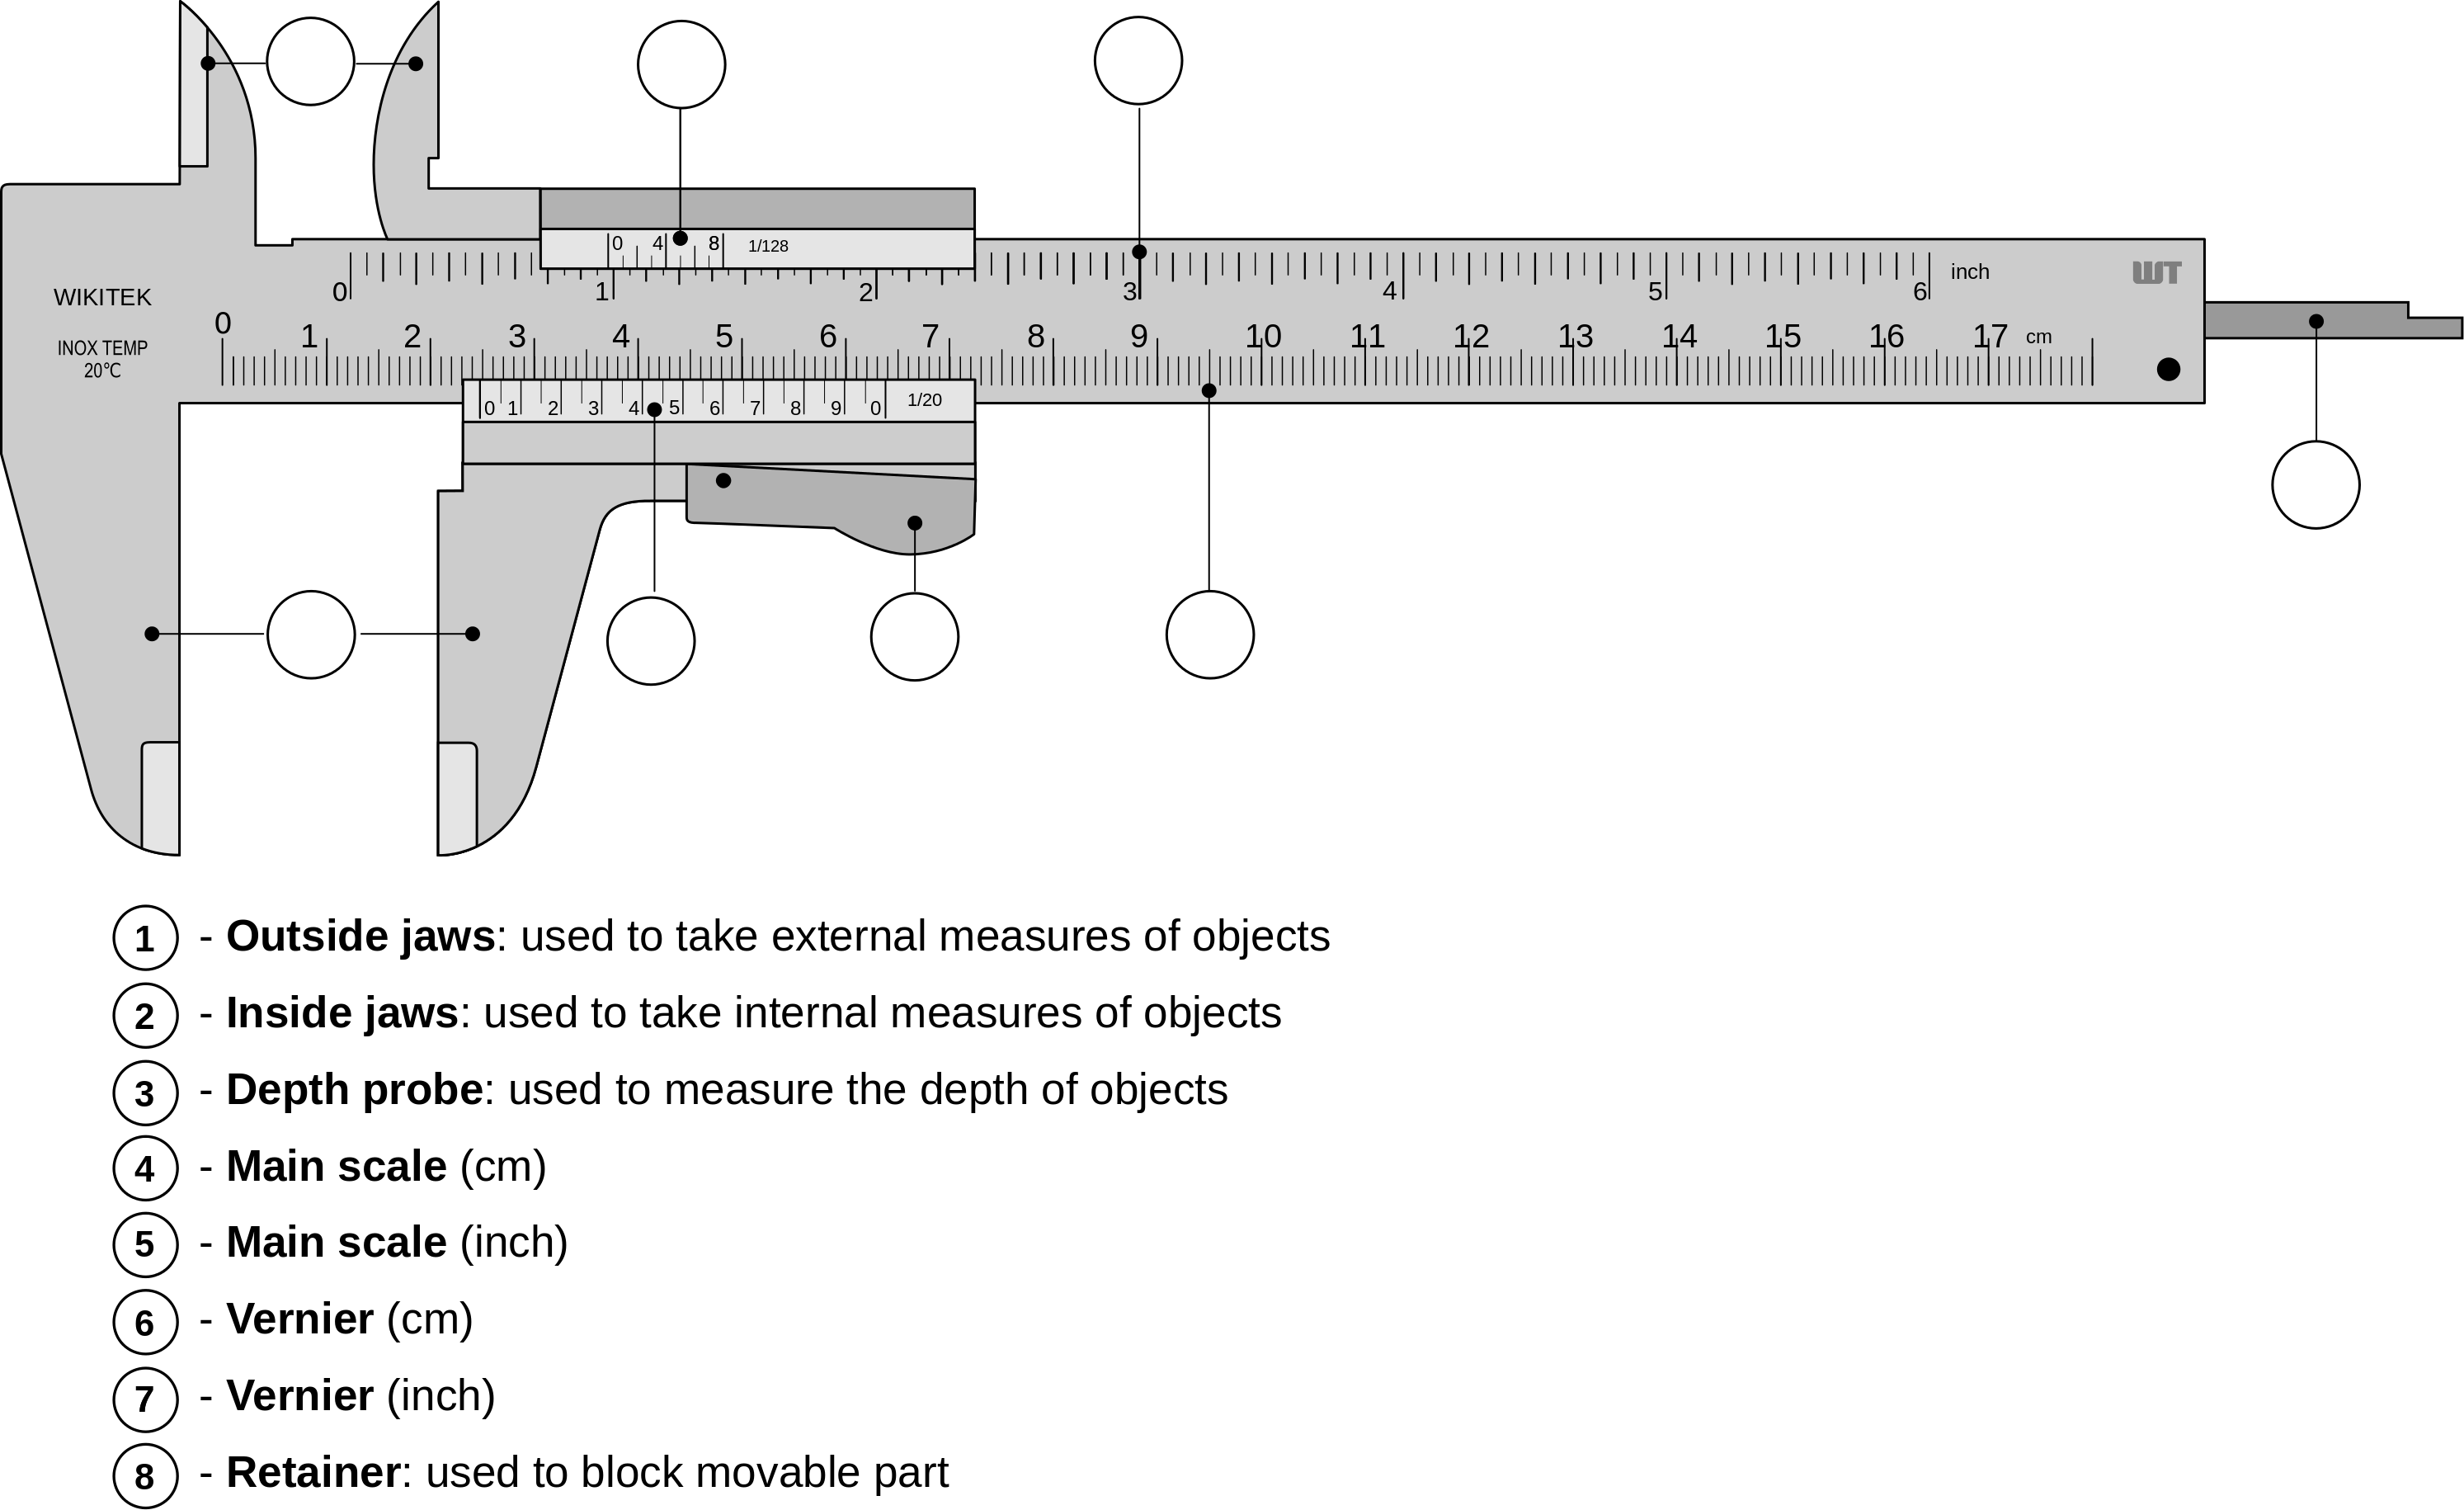
\includegraphics[scale=.08]{images/calipers_fig1.png}

			\end{frame}


		% section I subsection III
		\subsection{\sectionIsubsectionIIItitle}\label{sectionIsubsectionIII}
			\begin{frame} 
				\frametitle{\sectionIsubsectionIIItitle}
					\scriptsize	

					A vernier scale is a visual aid to take an accurate measurement reading between two graduation markings on a linear scale by using mechanical interpolation; thereby increasing resolution and reducing measurement uncertainty by using Vernier acuity to reduce human estimation error. \vspc

					\includegraphics[scale=.07]{images/vernier_calipers_fig1_cropped.png}

			\end{frame}	

		% section I subsection IV
		\subsection{\sectionIsubsectionIVtitle}\label{sectionIsubsectionIV}	

			\begin{frame}
				\frametitle{\sectionIsubsectionIVtitle}

				\scriptsize
				\begin{multicols}{2}
				\begin{enumerate}
				\item Inspect the jaws. Wipe the jaws with a clean rag or cloth. \vspcc

				\item Close the jaws around the object gently and avoid deflecting the object. Verify the reading is zero. \vspcc

				\item Read the main scale and record the measurement. \vspcc

				\item Read the Vernier scale and add to the main scale measurement. \vspace{8mm}\\
				\end{enumerate}


				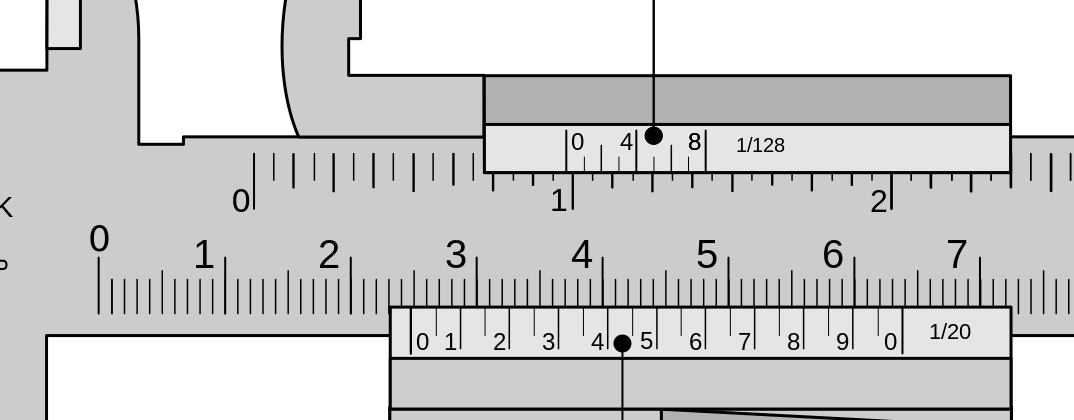
\includegraphics[scale=.15]{images/calipers_fig1_cropped.png}
				\end{multicols}
		

			\end{frame}



	% Section II
	\section{\sectionIItitle}\label{sectionII}

		% section II Outline
		\begin{frame}
			\large \textbf{Topic 2 - \sectionIItitle} \vspace{3mm}\\

			\begin{itemize}
				\item \hyperlink{sectionIIsubsectionI}{\sectionIIsubsectionItitle} \vspc %  section II subsection I
				\item \hyperlink{sectionIIsubsectionII}{\sectionIIsubsectionIItitle} \vspc % section II subsection II
				\item \hyperlink{sectionIIsubsectionIII}{\sectionIIsubsectionIIItitle} \vspc % section II subsection III
				\item \hyperlink{sectionIIsubsectionIV}{\sectionIIsubsectionIVtitle} \vspc % section II subsection IV
			\end{itemize}
		\end{frame}

		% section II subsection I
		\subsection{\sectionIIsubsectionItitle}\label{sectionIIsubsectionI}

			\begin{frame}[label=sectionIIsubsectionI]
				\frametitle{\sectionIIsubsectionItitle}

				A micrometer, sometimes known as a micrometer screw gauge, is a device incorporating a calibrated screw widely used for accurate measurement of components[1] in mechanical engineering and machining as well as most mechanical trades, along with other metrological instruments such as dial, vernier, and digital calipers. {\tiny Text: \href{https://en.wikipedia.org/wiki/Micrometer}{Wikipedia}}\vspc

				Unlike a pair of Vernier or digital calipers, most micrometers are designed to measure outside dimensions only. \vspc

				{\tiny Text: \underline{Theory and Design of Mechanical Measurements, 5th Edition}}
	
			\end{frame}

		% section II subsection II
		\subsection{\sectionIIsubsectionIItitle}\label{sectionIIsubsectionII}

			\begin{frame}
				\frametitle{\sectionIIsubsectionIItitle}
				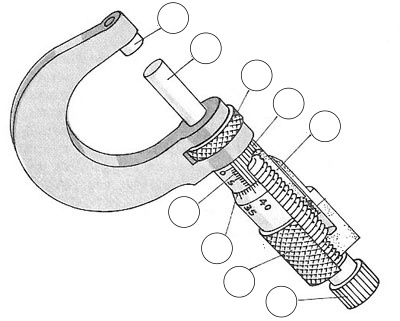
\includegraphics[scale=.35]{images/micrometer_fig2.png}
		        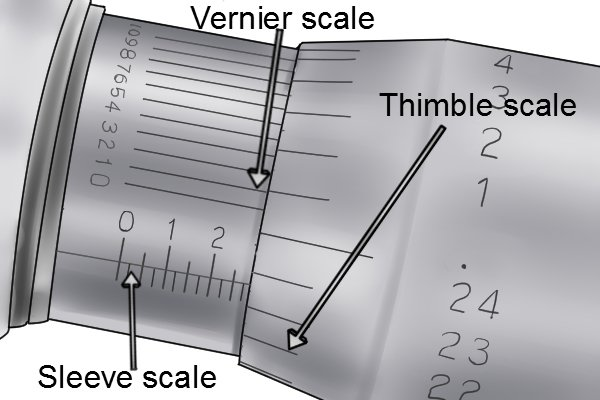
\includegraphics[scale=.25]{images/micrometer_fig1.png}
		        \begin{multicols}{2}
		        	\begin{enumerate}
		 			\item Anvil
		 			\item Spindle
		 			\item Thimble
		 			\item Lock Ring
		 			\item Sleeve Scale
		 			\item Thimble Scale
		 			\item Vernier Scale
		 			\item Ratchet (Clutch) Knob			
		 		\end{enumerate}
		 		\end{multicols}


			\end{frame}

		% section II subsection III
		\subsection{\sectionIIsubsectionIIItitle}\label{sectionIIsubsectionIII}

			\begin{frame}
				\frametitle{\sectionIIsubsectionIIItitle}

				A vernier scale is a visual aid to take an accurate measurement reading between two graduation markings on a linear scale by using mechanical interpolation; thereby increasing resolution and reducing measurement uncertainty by using Vernier acuity to reduce human estimation error.  {\tiny \href{https://en.wikipedia.org/wiki/Vernier_scale}{Wikipedia}}

				\begin{multicols}{2}
				\underline{Pros}
				\begin{itemize}
				\item 
				\item
				\item
				\end{itemize}
				\underline{Cons}
				\begin{itemize}
				\item 
				\item
				\item
				\end{itemize}
				\end{multicols}

			\end{frame}

		% section II subsection IV 
		\subsection{\sectionIIsubsectionIVtitle}\label{sectionIIsubsectionIV}

			\begin{frame}
				\frametitle{\sectionIIsubsectionIVtitle}
				A digital micrometer contains an embedded processor and user interface to facilitate the measurement process.

				\begin{multicols}{2}
				\underline{Pros}
				\begin{itemize}
				\item 
				\item
				\item
				\end{itemize}
				\underline{Cons}
				\begin{itemize}
				\item 
				\item
				\item
				\end{itemize}
				\end{multicols}
		

				Make sure to clean the jaws and zero the instrument before you take a measurement. Also, be careful not to press the zero button on accident. On some models this is very easy to do. \vspace{40mm}\\

			\end{frame}


\end{document}





